\section{Auswertung}
\label{sec:Auswertung}
Der rechte Ausgang des Referenc/Oscillator gibt es eine konstante Spannung
von $2.4\si{\volt}$ der linke Ausgang liefert eine variable Spannung die
als Rechteck oder sinusförmige Spannung abgegeben werden kann. Für die
Phasenverschiebung $\Phi=0,0,0,0,0$ sehen die Signale wie in den folgenden
Bildern aus.
\begin{figure}
  \centering
  \begin{subfigure}{0.48\textwidth}
    \centering
    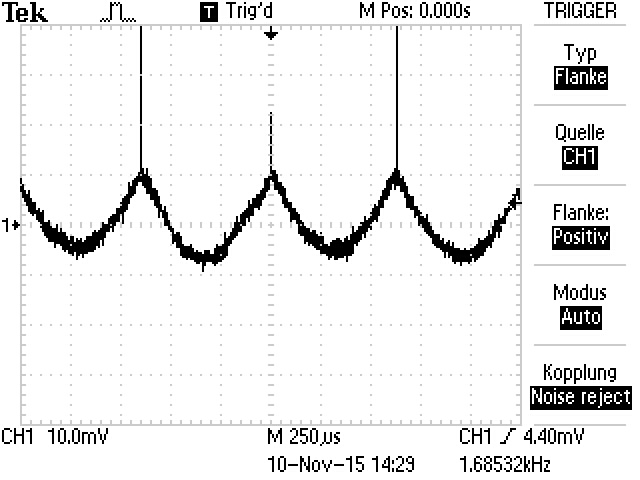
\includegraphics[height=0.75cm]{Bilder/or/or10.JPG}
    \caption{Phasenwinkel 10.}
    \label{fig:or10}
  \end{subfigure}
  \begin{subfigure}{0.48\textwidth}
    \centering
    %\includegraphics[height=0.75cm]{/pep.pdf}
    \caption{phasenwinkel 100.}
    \label{fig:pep2}
  \end{subfigure}  \centering
    \begin{subfigure}{0.48\textwidth}
      \centering
      %\includegraphics[height=0.75cm]{/pep.pdf}
      \caption{phasenwinkel 150.}
      \label{fig:pep2}
    \end{subfigure}
  \centering
  \begin{subfigure}{0.48\textwidth}
    \centering
    %\includegraphics[height=0.75cm]{/pep.pdf}
    \caption{phasenwinkel 190.}
    \label{fig:pep2}
  \end{subfigure}
  \begin{subfigure}{0.48\textwidth}
    \centering
    %\includegraphics[height=0.75cm]{/pep.pdf}
    \caption{phasenwinkel 280.}
    \label{fig:pep2}
  \end{subfigure}
\end{figure}
Wenn das Ausgangssignal über den Tiefpass für $\Phi=$ integriert wird sieht das
Signal aus wie in dem folgenden Bild.
\begin{figure}

\end{figure}
Die Messwerte Aus der Messung ohne Rauschen sind in folgender Tabelle aufgelistet
\begin{table}
  \centering
  \begin{tabular}{c c}
    \toprule
    $Spannung/V$  &  Phasenwinkel $\phi$\\
    \midrule
    24.8  &    0  \\
    22.8  &   30  \\
    15.7  &   60  \\
    12.0  &   90  \\
     5.7  &  120  \\
     1.3  &  150  \\
     0.8  &  180  \\
     3.2  &  210  \\
    10.4  &  240  \\
    14.2  &  270  \\
    20.6  &  300  \\
    24.8  &  330  \\
    25.0  &  360  \\
   \bottomrule
 \end{tabular}
 \caption{Differentialquotienten.}
 \label{tab:Diffquo}
\end{table}
